% rectangle, circle, arc


\documentclass{standalone}

%maths
\usepackage{tikz}
\usepackage{scalerel}
\usepackage{pict2e}
\usepackage{tkz-euclide}
\usetikzlibrary{calc}
\usetikzlibrary{patterns,arrows.meta}
\usetikzlibrary{shadows}
\usetikzlibrary{external}

%pgfplot

\usepackage{pgfplots}
\pgfplotsset{compat=newest}
\usepgfplotslibrary{statistics}
\usepgfplotslibrary{fillbetween}

%colours
\usepackage{xcolor}



\begin{document}



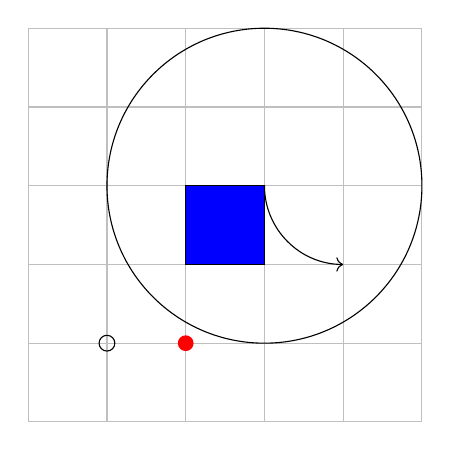
\begin{tikzpicture}

%circle
\draw[step = 1,  lightgray] (0,0) grid (5,5);

\draw (3,3) circle [radius = 2];   % circle
\draw (1,1) circle [radius = .1];  %works like a point
\fill[red] (2,1) circle [radius = .1];   % a filled circle


%rectangle

%\draw (2,2) -- (3,2) -- (3,3) -- (2,3) -- (2,2);
\draw (2,2) rectangle (3,3);     % does the same as previous line
\draw (2,2) rectangle (3,3); 
\fill[blue] (2,2) rectangle (3,3); 


%Arc

\coordinate (A) at (3,3);
\draw[->] (A) arc (0:90:-1);

% arc(a:b:c) -->> a = start angle(degrees), b = end angle, c = radius ;
  



\end{tikzpicture}


\end{document}